% allocate 18 pages
\chapter{Implementation}

Note: maybe include time complexity of each algo, for example Auto prompting:  in each epoch, assume $b$ batches of train dataset and validation dataset, then we require $b$ forward steps and $b$ backward steps in (a), assume $n$ candidate tokens, then computing the candidate set using HotFlip is like adding a language model output projection, then iterating all candidate tokens in (c) requires an additional $nb$ forward steps.

In the past decade, NLP tasks have relied on deep neural network architectures such as the convolutional neural networks (CNN) \cite{Krizhevsky12CNN, He15CNN, Han19CNN}. The introduction of transformers that are built on top of the self-attention mechanism 
 revolutionised the field \cite{Vaswani17attention}.

\subsubsection{Attention mechanism}
The characteristics of human perception inspired the attention mechanisms \cite{Bahdanau14attention}. Given a sentence, humans would concentrate on specific segments instead of processing the entire sentence \cite{Niu21attention}, and learn to focus on informative parts of the input text when faced with similar situations. In NLP, the attention mechanism is widely used in sequence-to-sequence models \cite{Chorowski15attention, Chan15attention, Bahdanau15attention} to provide a flexible encoding scheme. It is built on the encoder-decoder framework with recurrent neural networks (RNN) \cite{Cho14EncDec, Sutskever14EncDec}. 

\begin{figure}[!ht]
    \centering
    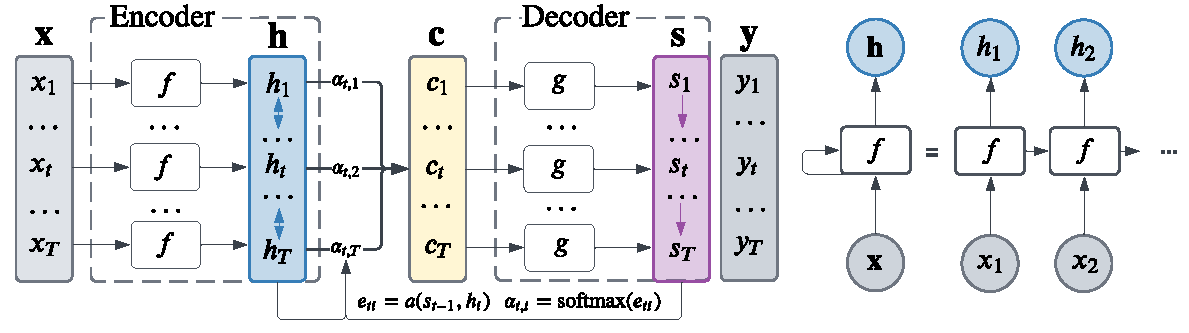
\includegraphics[width=\hsize]{figures/preparation_media/prepare-attention.pdf}
    \caption{The attention mechanism (left) is built on the encoder-decoder framework. RNN (right) facilitates neuron communication through signal transmission.}
    \label{fig:prepare-attention}
\end{figure}

The attention mechanism uses an encoder to map an input tokenised sequence $\textbf{x} = (x_1,...,x_T)$ to a contextualised vector $\textbf{c} = (c_1, ..., c_n)$ where $c_i$ captures the relevance between surrounding tokens and the current one at position $i$. The decoder then generates an output sequence $\textbf{y} = (y_1, ..., y_n)$ based on the contextualised vector $\textbf{c}$, one element at a time \cite{Vaswani17attention}. 

Formally, given an input tokenised sequence $\textbf{x} = (x_1,...,x_T)$, the encoder scans through the sequence, for each token $x_t$, generates a RNN hidden state $h_t$ based on previous history $h_{t-1}$ using a nonlinear RNN function $f$:
\begin{equation}
    h_t = f(x_t, h_{t-1})
\end{equation}
The attention mechanism uses a bidirectional RNN layer for the encoder, so both a forward hidden state $\overrightarrow{h}_t$ and a backward hidden state $\overleftarrow{h}_t$ are defined, where the backward RNN function $\overleftarrow{f}$ reads inputs in a reverse order.

The decoder is trained to predict output token $y_t$ based on the current context $c_t$ and the token prediction history $\{y_1, ..., y_{t-1}\}$, the probability likelihood of $y_t$ is written using a non-linear function $q$:
\begin{equation}
    \Pr(y_t| \{y_1, ..., y_{t-1}\}, \textbf{x}) = q(y_{t-1}, s_t, c_t)
\end{equation}
where $s_t$ is an RNN hidden state for output label $y_t$ and $c_t$ is a contextualised vector that encapsulates relationships between tokens at the current time stamp $t$. Contextualised vector $c_t$ is a weighted sum of hidden states $\textbf{h}$:
\begin{equation}
    c_t = \sum_{i=1}^T \alpha_{t,i}h_i = \sum_{i=1}^T \frac{\exp(e_{ti})}{\sum_{j=1}^T \exp(e_{tj})} h_i
\end{equation}
where weight $\alpha_{t,i}$ for each hidden state $h_i$ is the normalised score $e_{ti}$ that computes how well input tokens around position $t$ and output tokens around position $i$ match. We define score $e_{ti} = a(s_{t-1}, h_i)$ where alignment model $a$ is a feedforward neural network.

Conversely, the self-attention mechanism learns contextual relations between words in the single sentence  \cite{Vaswani17attention}, generating a new sequence representation for the input sequence.

\subsubsection{Transformers with self-attention}
Transformers is a neural network architecture that build from the self-attention mechanism, eliminates the RNN layers but preserves the encoder-decoder structure, to better maintain long-distance dependencies \cite{Kalyan21transformer}. 

Using a transformer model, the feature vectors generated in the feature extraction stage will be further projected by an embedding layer onto continuous dense vector representations, so-called contextualised word embeddings, which preserves the semantic meanings of the tokens in the context \cite{Almeida19wordembedding}. The embedding layer is initialised randomly and needs to be fine-tuned during model training. The embeddings generated will be fed as input into the encoder.

The encoder reads the entire input embeddings at once, instead of sequentially, allowing the model to learn the semantic meaning of the token based on all of its surroundings.
